\documentclass{article}
\usepackage{fancyhdr}
\usepackage{xeCJK}
\usepackage{pifont}
\usepackage{graphicx}
\usepackage{float}
\usepackage{geometry}
\geometry{left=1.5cm,right=1.5cm,top=3cm,bottom=3cm}
%\setmainfont{Times New Roman}  
\setCJKmainfont{Songti SC}
\pagestyle{fancy}
\fancypagestyle{plain}{
    \fancyhf{}
    \fancyfoot[C]{\thepage}
    \renewcommand\headrulewidth{0pt}
}
\begin{document}
    \noindent\textbf{2.6}\par
    地址空间大小为$2^{24}=16$MB,存储器组织如下图:\\
    \begin{figure}[h]
        \centering
        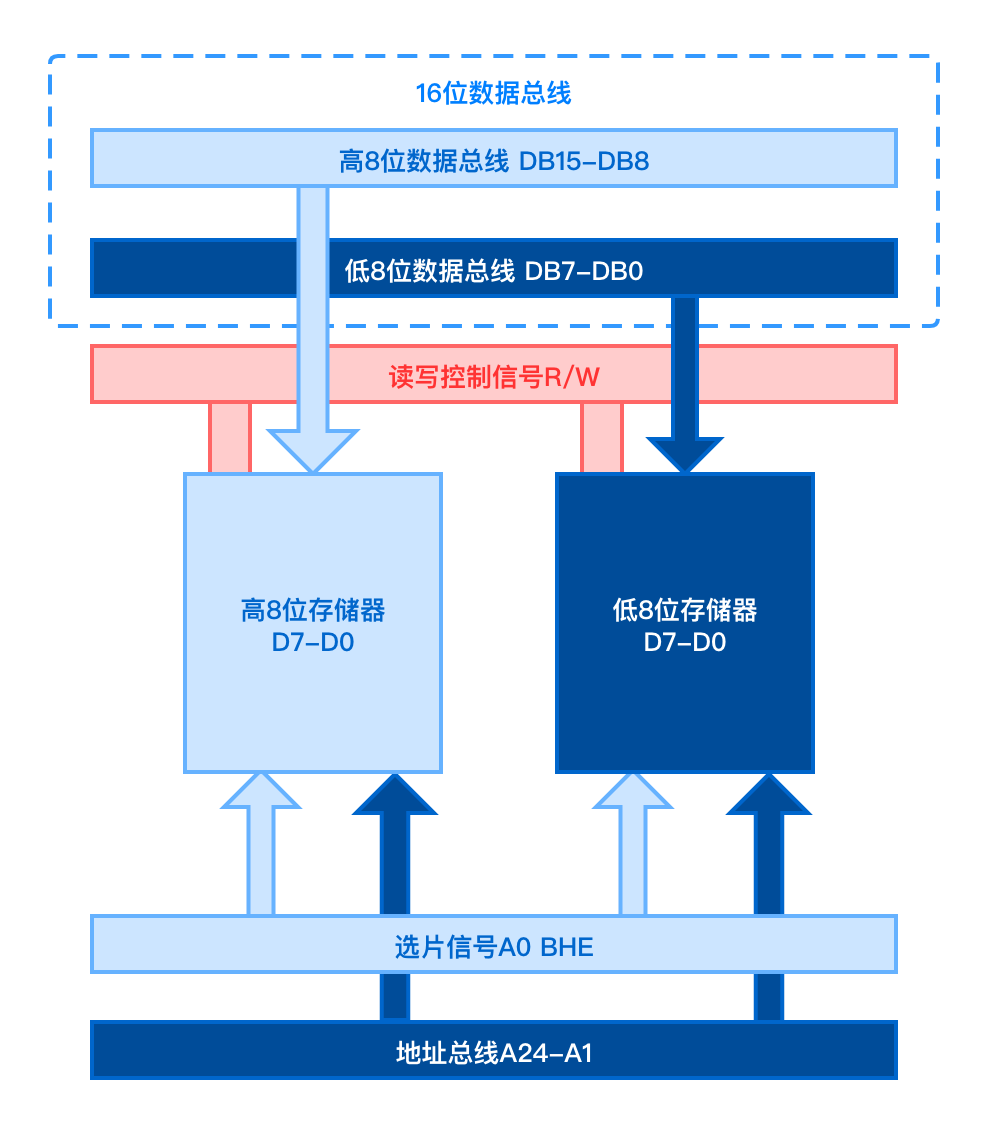
\includegraphics[scale=0.3]{hw2.png}
        \end{figure}
    \par
    使用两块存储器分别用于存储16位中的高8位和低8位;剩下的23位用来选择地址.如果需要操作完整的16位,则两片存储器同时操作;否则可以选择其中的一片来完成高8位或者低8位的读取.
    \\[4pt]\par

    \noindent\textbf{2.10}\par
    微指令指的是面向微程序级别的指令,用来描述微操作(相对于机器指令被机器直接读取、宏指令面向软件).\par
    一条(机器)指令对应了一个微程序,而一个微程序由多条微指令组成.\par
    在基于微程序设计的控制器中,每个微程序(其包括的微指令)都存放在控制ROM中,并且有唯一的(微)地址.译码器读取到指令操作码后开始在控制ROM中寻址,按顺序读出每一条微指令,产生控制信号,来执行微程序.
    \\[4pt]\par

    \noindent\textbf{2.13}\par
    \ding{172}程序计数器内容0x20000004送到地址生成部件,通过地址总线、到地址译码器进行译码,寻址这条指令.\par
    \ding{173}操作控制器从0x20000004读出内容“LDR R1,[R3]”,经过数据总线存入到指令寄存器IR中.\par
    \ding{174}程序计数器自增,准备读取下一条指令.\par
    \ding{175}指令译码器ID对操作数译码,操作控制器OC按时序发出相应控制信号.\par
    \ding{176}R1为目的操作数,[R3]为源操作数,[]表示间接读取存储器中的内容.\par
    \ding{177}控制信号按顺序执行,控制器在内存中寻找R3寄存器中存放地址,读取其中内容,存放到R1中.
    \\[4pt]\par

    \noindent\textbf{2.14}\par
    不能.\par
    为了叙述方便,不妨设a位存储器、b位地址总线,a<b.\par
    由于存储器单元都有b位的地址,在定长指令中无法用a位的地址码给出b位的源和目标地址,因此需要不止一个指令周期的寻址操作来进行寻址.
    \\[4pt]\par

    \noindent\textbf{2.15}\par
    \ding{172}WAW(Write After Write)\par
    \qquad I1:\qquad MOV\ R1,\#00000001\par
    \qquad I2:\qquad ADD\ R1,R1,\#00000002\par
    如果I2的写入在I1之前执行,那么结果R1里存的就是I1的结果\#1.但正确的逻辑结果应该是I2的ADD操作后的\#3.\\[2pt]\par
    \ding{173}WAR(Write After Read)\par
    \qquad I0:\qquad MOV\ R1,\#00000001\par
    \qquad I1:\qquad STR\ R1,[R3]\par
    \qquad I2:\qquad MOV\ R1,\#00000002\par
    如果I2的写入先于I1的读取,那么存入R3的数据就是I2中的\#2,但是程序的正确逻辑结果应该是I0中的\#1.
    \\[4pt]\par

    \noindent\textbf{2.16}\par
    \ding{172}转移指令跳转到的目标指令地址$I_k$\par
    \ding{173}假设从$I_j$跳转到$I_k$,则在流水线上,处理$I_j$时多需要三个周期,会导致$I_{j+1}$和$I_{j+2}$被装载到流水线上,造成两个流水线周期延迟.\par
    \ding{174}转移指令后面一个时间片\par
    \ding{175}转移目标缓冲器,收集储存近期所有转移信息并打表;转移时查表进行操作
    \\[4pt]\par

    \noindent\textbf{2.18}\par
    原因:必须保证每条流水线上的指令不相干.\par
    例如:\par
    \qquad I1:\qquad MOV\ R1,\#00000001\par
    \qquad I2:\qquad ADD\ R1,R1,\#00000002\par
    两条指令用到牵扯到对同一个寄存器的改写,因此不能在不同的流水线上并行.
    \\[4pt]\par

    \noindent\textbf{2.20}\par
    \ding{172}同构多核处理器指多核的每一个内核采用相同的结构、地位相等,简单增加处理器数量.\par
    \ding{173}异构多核处理器指配置不同功能和性能的内核来匹配实际应用需求,提升芯片总体性能的同时优化处理器结构、降低系统功耗.\par
    举例:通过将CPU和GPU集成到一颗芯片上,形成异构多核,串行执行部分在CPU上处理,并行部分在GPU上处理,以此来提升处理速度.
    \\[4pt]\par

    \noindent\textbf{2.24}\par
    1.1MIPS/MHz $\times$ 300MHz=330MIPS
    \\[4pt]\par

    \noindent\textbf{2.25}\par
    不能.例如,对于RISC和CISC,相同的任务下前者花费指令更多,因此MIPS不能简单地作为唯一评判指标.
    \\[4pt]\par

\end{document}